%File: formatting-instruction.tex

\documentclass{sig-alternate-2013}
\newfont{\mycrnotice}{ptmr8t at 7pt}
\newfont{\myconfname}{ptmri8t at 7pt}
\let\crnotice\mycrnotice%
\let\confname\myconfname%

\permission{Permission to make digital or hard copies of part or all of this work for personal or classroom use is granted without fee provided that copies are not made or distributed for profit or commercial advantage, and that copies bear this notice and the full citation on the first page. Copyrights for third-party components of this work must be honored. For all other uses, contact the owner/author(s). Copyright is held by the author/owner(s).}
\conferenceinfo{HRI'15 Extended Abstracts,}{March 2--5, 2015, Portland, OR, USA.} 
\copyrightetc{ACM \the\acmcopyr}
\crdata{978-1-4503-3318-4/15/03. \\
http://dx.doi.org/10.1145/2701973.2702710}

\clubpenalty=10000 
\widowpenalty = 10000


% Load basic packages
\usepackage{balance}  % to better equalize the last page
\usepackage{url}      % llt: nicely formatted URLs

\usepackage{times}
\usepackage{helvet}
\usepackage{courier}
\usepackage{graphicx}
\usepackage{subcaption}

\usepackage{amsfonts}
\usepackage{amsmath}
\usepackage{algorithmicx}
\usepackage{algpseudocode}
\usepackage{algorithm}


% llt: Define a global style for URLs, rather that the default one
\makeatletter
\def\url@leostyle{%
  \@ifundefined{selectfont}{\def\UrlFont{\sf}}{\def\UrlFont{\small\bf\ttfamily}}}
\makeatother
\urlstyle{leo}

% To make various LaTeX processors do the right thing with page size.
\def\pprw{8.5in}
\def\pprh{11in}
\special{papersize=\pprw,\pprh}
\setlength{\paperwidth}{\pprw}
\setlength{\paperheight}{\pprh}
\setlength{\pdfpagewidth}{\pprw}
\setlength{\pdfpageheight}{\pprh}

% Make sure hyperref comes last of your loaded packages, 
% to give it a fighting chance of not being over-written, 
% since its job is to redefine many LaTeX commands.
\usepackage[pdftex]{hyperref}
\hypersetup{
pdftitle={SIGCHI Conference Proceedings Format},
pdfauthor={LaTeX},
pdfkeywords={SIGCHI, proceedings, archival format},
bookmarksnumbered,
pdfstartview={FitH},
colorlinks,
citecolor=black,
filecolor=black,
linkcolor=black,
urlcolor=black,
breaklinks=true,
}


\DeclareMathOperator*{\argmin}{argmin}

%\makeatletter
%\let\@copyrightspace\relax
%\makeatother

% if you are using PDF LaTex and you cannot find a way for producing
% letter, the following explicit settings may help

%\pdfpagewidth=8.5truein
%\pdfpageheight=11truein

\begin{document}


%\TitleForCitationInfo{Extending the Difference Reward to Multi-Objective Reinforcement Learning}

\title{Developing Learning from Demonstration Techniques for Individuals with Physical Disabilities}


\author{William Curran \\
Oregon State University \\
Corvallis, Oregon \\
curranw@onid.orst.edu \\
}
%\And
%Adrian Agogino \\
%NASA AMES Research Center \\
%Moffet Field, California \\
%adrian.k.agogino@nasa.gov \\
%\And 
%Kagan Tumer \\
%Oregon State University \\
%Corvallis, Oregon \\
%kagan.tumer@oregonstate.edu \\
%}

\maketitle

\begin{abstract}

%CARRIE'S BEGINNING OF EDITS: Most research in learning from demonstration assumes that the demonstrator can move quickly to give feedback or demonstrations. This work develops interfaces and tools to enable persons with severe motor disabilities to train learning systems.

Learning from demonstration research often assumes that the demonstrator can quickly give feedback or demonstrations. Individuals with severe motor disabilities are often slow and prone to human errors in demonstrations while teaching. Our work develops tools to allow persons with severe motor disabilities, who stand to benefit most from assistive robots, to train these systems. To accommodate slower feedback, we will develop a movie-reel style learning from demonstration interface. To handle human error, we will use dimensionality reduction to develop new reinforcement learning techniques.

%In learning from demonstration research, there's often an implicit assumption that the demonstrator is able to move in a timely manner, either to give feedback or demonstrations. This work relaxes this assumption, with interfaces and tools that explicitly allow for persons with severe motor disabilities, who stand to benefit most from assistive robots, to train these systems. Additionally, individuals with severe motor disabilities are more prone to human errors in demonstrations while teaching. 

%In this work we will develop a movie-reel style learning from demonstration interface that removes the need for timely feedback. We will also develop reinforcement learning techniques that are both robust to supoptimal outliers in demonstrations and require fewer overall demonstrations.

%The field of Human-Robot Interaction (HRI) has recently emerged as an area of research dedicated to understanding and evaluating robotic systems to be used by humans. Traditionally, HRI has focused on a psychological analysis of how an able-bodied individual can cooperatively accomplish tasks with a robot. Our work removes the assumption that the user is able-bodied, and focuses on developing interfaces and reinforcement learning tools for people with amyotrophic lateral sclerosis (ALS) and quadriplegia to effectively teach and use a personal assistant robot. 

%Those suffering from ALS and quadriplegia need robots in the world now, and cannot wait for an expert to develop autonomy of every task. By using a teaching approach, we will develop a learning from demonstration algorithm that allows those with severe physical disabilities to teach custom routines to the robot and give accurate feedback to guide the learning. 



%We will then develop a goal-based interface, allowing users to use Google Glass to semantically map objects in their home. Combining the high level tasks learned through demonstration, and the semantic information obtained during object classification, we can build a new interface allowing users to give high level goals to a group of robots.

%The Robot Interactive Display Environment (RIDE) interface was built to allow one user to control multiple robots at different fidelity levels. We will expand RIDE to allow users to teach the robot by demonstration through a shared autonomy system in combination with Google Glass, Oculus Rift and Razer Hydra. We will create two custom interfaces, one being hands-free with Google Glass and the other using the Oculus Rift and Hydra.
\end{abstract}


\section{Introduction}
The main goal for our research is to put robots into real homes to help those with severe physical disabilities. These
individuals have minimal ability to move and speak, and need extended care all day, every day. The strain on families needing to take care of these individuals is enormous, and it has been shown that inexperienced family caregivers use prescription drugs for depression, anxiety, and insomnia two to three times more often than the average population \cite{Gallagher01081989}. Robotics can be used to assist those with extreme disabilities and remove much of this burden on the family.

These disabled individuals are often non-experts, and currently cannot be part of the development process. Yet, most don't want to wait for someone to program autonomous behaviors for all household tasks. We propose to give disabled non-expert users the tools to teach the robot these tasks by themselves. This will give the disabled user both independence and personal customization.

%We promote using a learning from demonstration approach to allow disabled users to teach their assistive robot. Using demonstrations to initialize reinforcement learning provides supervised training data of what actions to perform in states that are encountered \cite{Bagnell_2013_7451}. Using this initialization, the robot can perform the task to a small degree, and the user can take the role of a teacher, giving feedback.

We use a learning from demonstration approach to allow disabled users to teach their assistive robot. In learning from demonstration, users show the robot what actions to execute to perform a task. These user demonstrations are training data for the reinforcement learning algorithm \cite{Bagnell_2013_7451}. Using this initialization, the robot can attempt to perform the task, and the user can give feedback as a teacher. Good demonstrations and timely feedback are key assumptions in learning from demonstration approaches \cite{Argall:2009:SRL:1523530.1524008}. However, our user base is people who suffer from severe physical disabilities. They can't provide a good or timely demonstrations or feedback to guide the learning. These individuals need specially designed interfaces and tools.

%However, our user base is people who suffer from severe physical disabilities. These individuals require specially designed interfaces and tools. This work will look at how to apply learning from demonstration for people who can't provide a good or timely demonstrations, and who cannot provide timely feedback to guide the learning.

%There are two key difficulties with learning from demonstration interfaces for individuals with disabilities, and resolving them are the key contributions of this work. The ability to perform good demonstrations and give timely feedback are key assumptions in learning from demonstration research \cite{Argall:2009:SRL:1523530.1524008}. Additionally, state-of-the-art personal robots need to perform complex manipulation tasks to be viable in assistive scenarios. These complex robots lead to large dimensional state spaces, known as the curse of dimensionality \cite{Bagnell_2013_7451}. 

%Good demonstrations and timely feedback are key assumptions in learning from demonstration research \cite{Argall:2009:SRL:1523530.1524008}. 

State-of-the-art personal robots also need to perform complex manipulation tasks to be viable in assistive scenarios. These complex manipulations need high degree-of-freedom arms and manipulators. The complexity of these robots lead to large dimensional state spaces, which are difficult to learn in. Additionally, the generalization of motor skills to similar tasks become especially important when demonstrations are difficult to perform. This also becomes more difficult in higher-dimensional state spaces. 

%To alleviate these issue, we promote developing a movie-reel style interface for detailed, yet time insensitive feedback. We also wish to analyze the efficacy of transforming a high-dimensional demonstration to a low-dimensional space, performing reinforcement learning in that space, and executing the learned trajectory back in the high-dimensional space. 

The contributions of the completed work will be to develop a movie-reel style interface for detailed, time insensitive feedback. This gives the user as much time as they need for demonstrations and feedback. We will also develop a robust, generalizable, and fast learning from demonstration technique. We transform a high-dimensional demonstration to a low-dimensional space. We then perform reinforcement learning in that space, and then execute the learned trajectory back in the high-dimensional space. This reduces the number of demonstrations and increases the resistance to suboptimal outliers. These are desirable characteristics for non-expert use of the learning algorithm.

\section{Related Work}
Developing a trajectory using traditional reinforcement learning does not work well in robotics. Finding an optimal or near-optimal solution requires exploration throughout much of the state space. Excessive exploring of the unknown state space risks damaging the robot. Small steps during exploration avoids this problem, but this brings the additional problem of taking longer to find an optimal solution. Initializing, or bootstrapping, the trajectory close to the desired robot behavior removes many of these problems. One approach to this initialization is learning from demonstration.

One current learning from demonstration research focus is on generalizing motor skills to similar tasks. Pastor et al. uses dynamic motor primitives to perform movement generation and generalization to a new goal \cite{Pastor_ICRA_2009}. However, this approach does not work well with uncertainty. Lee et al. developed belief space learning from demonstration techniques, taking into account uncertainty during learning \cite{Leeetal_IROS2013}. In current research, learning from demonstration requires the human teacher to map their movement directly to the joint angles of the robot and assumes an able-bodied user \cite{Bagnell_2013_7451}.

\section{Learning from Demonstration Interfaces}
\label{Learning by Demonstration}
%The Robot Operating System (ROS) \cite{quigley:ros} is becoming increasingly-widely used in the robotics research community. In this work we will use RViz, a ROS package that assists users in the visualization of robotic movements and sensors.  Our first focus of research is to extend RViz to be an interface for learning from demonstration.  

We need to develop a learning from demonstration interface that allows disabled users to teach their assistive robot at their own speed. We propose two interfaces: an early interface for super users, and one for users with severe physical disabilities. In this work we will use RViz, a ROS \cite{quigley:ros} package that assists users in the visualization of robotic movements and sensors.  Our first focus of research is to extend RViz to be an interface for learning from demonstration. 

%The interface for users without disabilities will take advantage of the direct first-person control aspect of RViz and the usability of the Oculus Rift (Figure ~\ref{Rift}) and Razer Hydra (Figure ~\ref{Hydra}) control systems. The Oculus Rift allows a user to see through the sensors of the robot, while the Hydra can compute the exact location and orientation of controllers in your hand, allowing the user direct control over robotic arms. Using these tools the user can efficiently teach the robot through demonstration.
The interface for users without disabilities will take advantage of the direct first-person control aspect of RViz.  We will also use the Oculus Rift and Razer Hydra control systems. The Oculus Rift allows a user to see through the sensors of the robot, while the Hydra controls the robot. The Hydra control system computes the exact location and orientation of controllers in your hands, allowing the user natural control of the robotic arms. Using these tools the user can efficiently teach the robot through demonstration.

%With disabilities: Robot will simulate itself doing the task, allowing rewind/fast forward, and user can pick correct/incorrect frames and actions.
%The interface for users with disabilities will use a less direct approach. The robot will come with a motion library of basic autonomous functions, such as turning knobs and picking up objects. First, the user will give the robot a sequence of these high level actions to accomplish the overall task. The robot will simulate itself doing the task in RViz. We will extend RViz to give a movie reel style interface, allowing rewinding and fast forwarding of the robot's simulation. The user can then provide feedback on an action or set of actions at his or her own speed. To combine the autonomous and learned routines the robot will be applying hierarchical reinforcement learning  \cite{Barto:2003:RAH:608557.608576}. This shared autonomy approach allows the users to build custom routines for the robot to perform in a timely manner without direct knowledge of the reinforcement learning algorithm.

The interface for users with disabilities will use a less direct approach. The robot will come with a motion library of basic autonomous functions, such as turning knobs and picking up objects. First, the user will give the robot a sequence of these high level actions to perform the task. The robot will simulate itself doing the task in RViz. We will extend RViz with a movie-reel style interface for rewinding and fast forwarding of the robot's simulation. The user can then provide feedback on an action or set of actions at his or her own speed. This learning from demonstration interface allows the users to build custom routines for the robot without direct knowledge of the reinforcement learning algorithm.

%\section{Semantic Mapping with Glass}
%\label{Object Classification}
%Glass can be used to classify objects in the world. Shared automation. The user labels objects, the robot remembers them and can then apply that knowledge during tasks. Task interface would be ride++, possibly in combination with Glass? Add a citation to Smart's work with Henry, if possible.
%Google Glass (Figure \ref{Glass}) is a wearable computer with a head-mounted display and camera. It can be used hands-free through voice commands, making it ideal for users with disabilities. It can be used as a computer vision tool to classify objects in the world, but without an extensive personal database it cannot know the semantic meaning of all of the objects a user wants to classify. 

%\begin{figure}
%\centering
%\begin{subfigure}{0.25\columnwidth}
%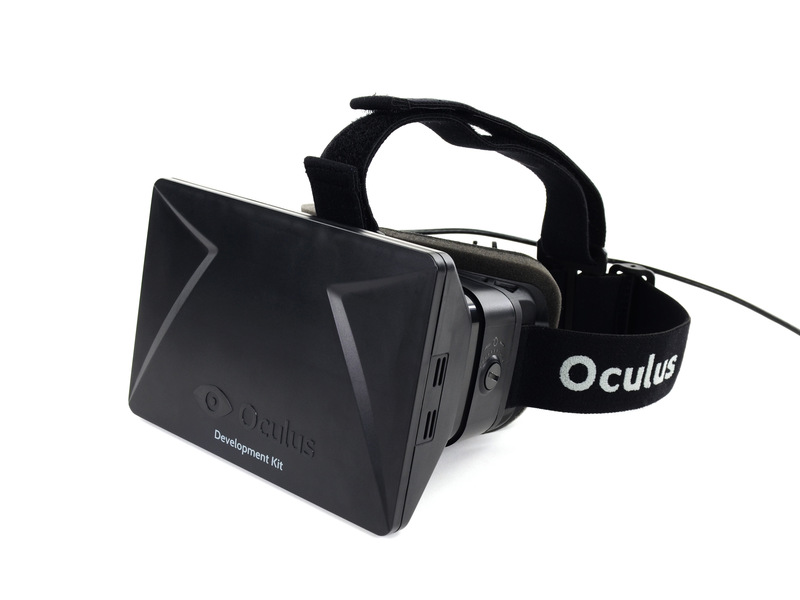
\includegraphics[width=1.0\columnwidth]{Oculus-Rift-1}
%\caption{Oculus Rift}
%\label{Rift}
%\end{subfigure}
%\begin{subfigure}{0.25\columnwidth}
%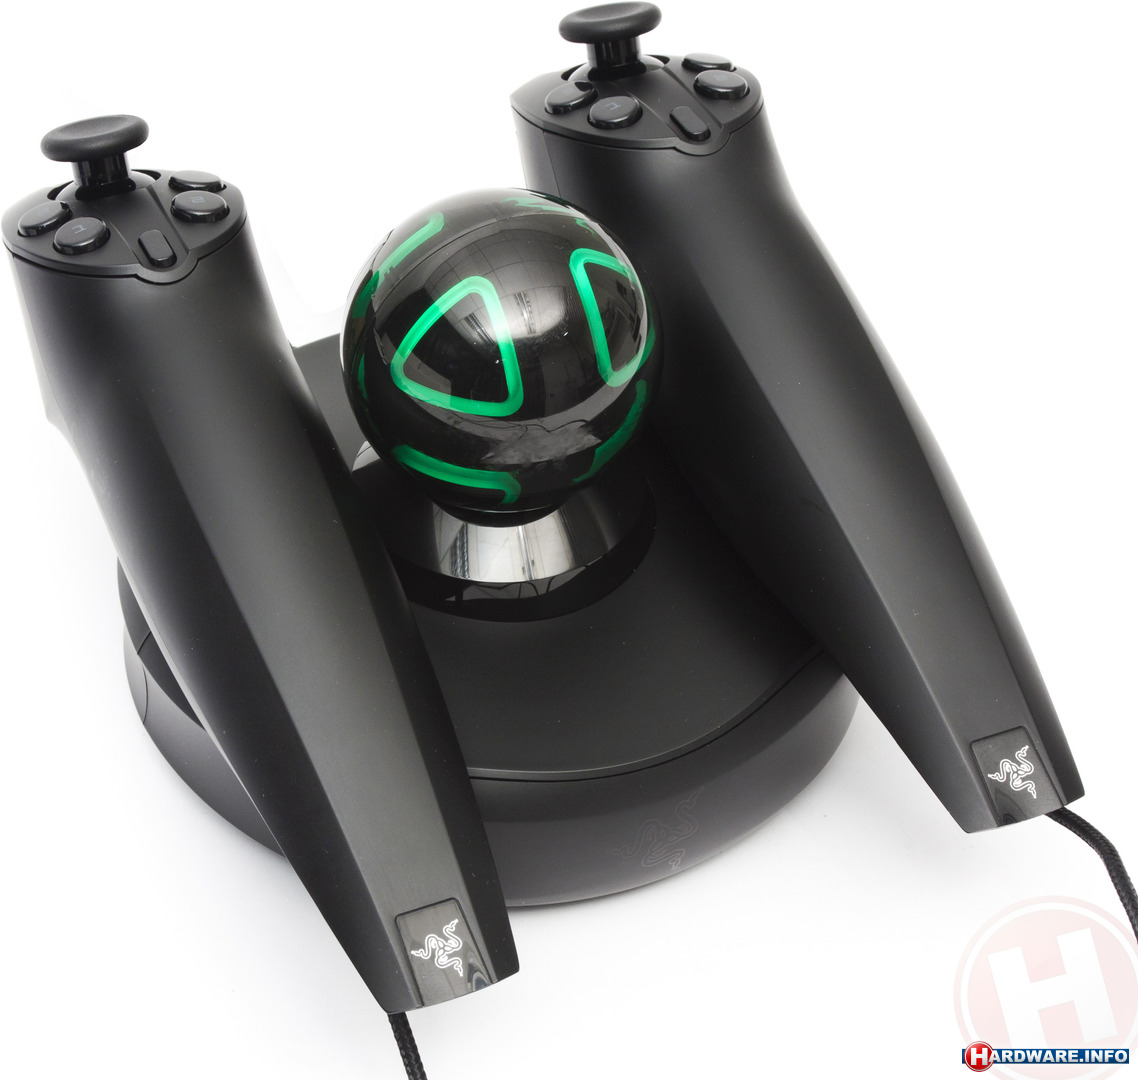
\includegraphics[width=1.0\columnwidth]{razer_hydra__portal_2}
%\caption{Razer Hydra}
%\label{Hydra}
%\end{subfigure}
%\begin{subfigure}{0.25\columnwidth}
%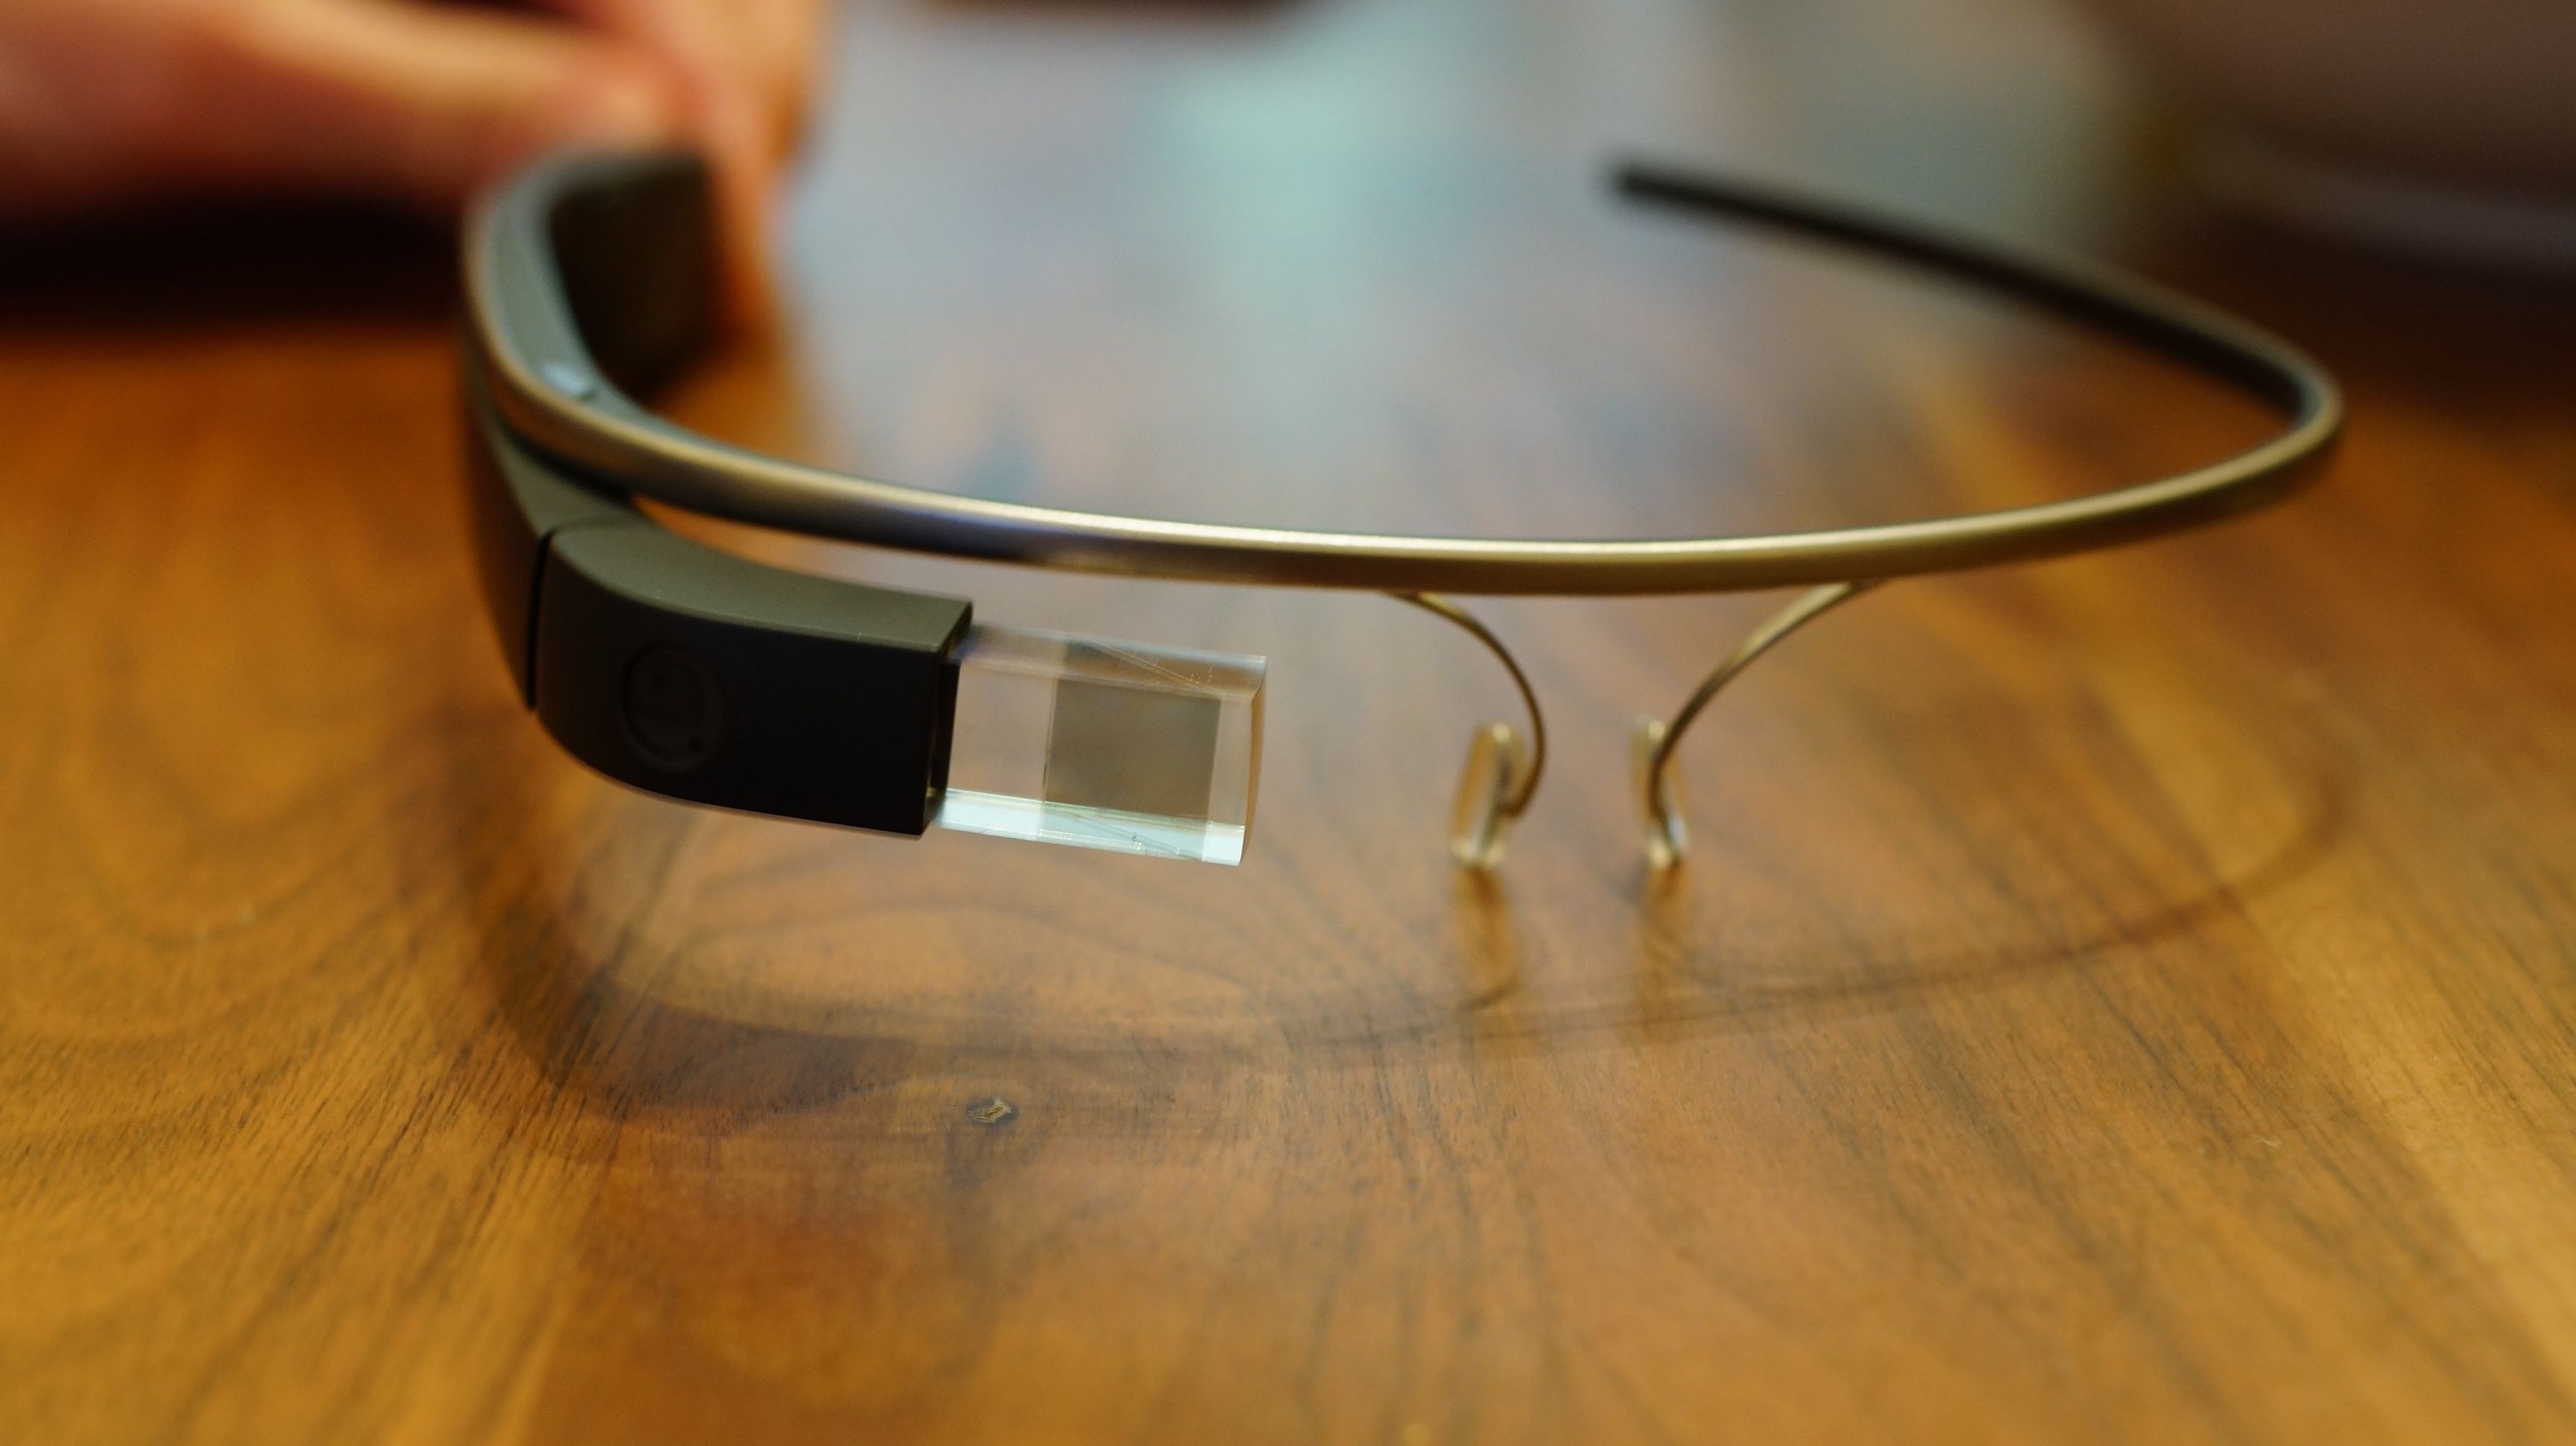
\includegraphics[width=1.0\columnwidth]{Google_Glass_Explorer_Edition}
%\caption{Google Glass}
%\label{Glass}
%\end{subfigure}
%\caption{State-of-the-art hardware tools for providing effective demonstrations.}
%\end{figure}

%We plan on developing a shared autonomy interface wherein the user can label objects using the Glass interface, and have that semantic mapping wirelessly sent to the robot. This semantic mapping can then be used as additional information when learning by demonstration and when giving tasks to the robot.

%For example, Google Glass can easily positively classify a desk, but it cannot know whose desk it is, or what the desk is used for. The user can tell Google Glass that this particular desk is his work desk, and when later gives a task to the robot to bring a book to his work desk, the robot will already have this semantic information.

\section{Learning from Demonstration in High-Dimensional Spaces}
\label{LfD in HD}
%State-of-the-art personal robots need to perform complex manipulation tasks to be viable in assistive scenarios. These complex manipulations require high degree-of-freedom arms and manipulators. For example, the PR2 robot is built with two 7 DoF arms. When learning position, velocity and acceleration control, this leads to a 21 dimensional state space for a single arm. Learning in these large dimensional spaces quickly becomes computationally intractable without optimization techniques. Furthermore, personal robots need to generalize learned motor skills between similar tasks, which in these high dimensional spaces also quickly becomes difficult \cite{Pastor_ICRA_2009}.

State-of-the-art personal robots need to perform complex manipulation tasks to be viable in assistive scenarios. These complex manipulations need high degree-of-freedom arms and manipulators. For example, the PR2 robot has two 7 DoF arms. When learning position, velocity and acceleration control, this leads to a 21 dimensional state space per arm. Learning in these large dimensional spaces becomes computationally intractable without optimization techniques. Furthermore, personal robots need to generalize learned motor skills between similar tasks. This also becomes difficult in these high-dimensional spaces \cite{Pastor_ICRA_2009}.

%To handle these high-dimensional spaces, our plan is to first perform dimensionality reduction (e.g. Principal Component Analysis) on a set of trajectories the user demonstrated to the robot while performing a task. We then transform the high-dimensional space to the first principal component, learn trajectories using the new subspace, and transform back to the high-dimensional space. By transforming to a smaller subspace, learning from demonstration techniques will converge faster to a solution.

To handle these high-dimensional spaces, our plan is to first perform dimensionality reduction on a set of demonstrated trajectories. We will use Principal Component Analysis to transform the high-dimensional space to a subspace. We then learn trajectories using the new subspace, and transform back to the high-dimensional space. By transforming to a smaller subspace, learning from demonstration techniques will converge faster to a solution.

%In addition to faster learning, we hypothesize that transforming trajectories to a lower dimensional space will allow us to more efficiently parameterize the task-based motor primitives. By parameterizing the motor primitives, we will be able to generalize motor skills to similar tasks, reducing the number of different demonstrations required. Additionally, we know that transforming to a lower dimensional space essentially smooths the trajectory. We hypothesize that this makes the learning more robust to suboptimal outliers caused by human error in the demonstration. 

By parameterizing the motor primitives, we will be able to generalize motor skills to similar tasks.  This will reduce the number of different demonstrations required. We hypothesize that transforming trajectories to a lower dimensional space will make it easier to parameterize the task-based motor primitives. Additionally, dimensionality reduction smooths the lower-dimensional trajectory. We hypothesize that this makes the learning more robust to suboptimal outliers caused by human error. Increasing the robustness to human error in demonstrations and reducing the number of demonstrations are essential. Since we work with individuals with disabilities, demonstrations are difficult, and expect suboptimal demonstrations. Since demonstrations are difficult, fewer demonstrations are also a desirable quality.

%Preliminary work has shown that while performing a complex sheet folding task, the first principal component represents 58\% and 33\% of the variance in position and velocity. Additionally, first three principal components represent 85\% of all of the variance in the position data and 75\% of all of the variance in velocity data. This reinforces the hypothesis that we can reduce the high-dimensional state space to a lower-dimensional space and still represent most of the given trajectory.

Preliminary work has shown that while performing a complex sheet folding task, the first principal component represents 58\% and 33\% of the variance in position and velocity. Additionally, first three principal components represent 85\% of all the variance in the position data and 75\% of all the variance in velocity data. This reinforces the hypothesis that we can represent a high-dimensional trajectory in a low-dimensional space.


%\section{Multi-Robot Coordination}
%Our final goal is multirobot interaction. RIDE was built to allow one user to control many robots directly. I want to make these tasks higher level. The user will be able to click on two robots, and right click an object. They see an interface with available actions, and the robots coordinate to accomplish that action. This is learned through a combination of demonstration and hierarchical learning (cite hierarchical learning paper. Maybe Q-MAX?).

%This can be extended to Glass. Rather than clicking on two robots, glass can be used in combination with a projector interface (Like Dan's work) for people with disabilities.

%RIDE was originally created to allow one user to control many robots directly, or take a supervisory role. However, the current supervisory role can be expanded to include giving high level goals, such as bringing the user a book. Combining the abilities learned through demonstration in Section \ref{Learning by Demonstration} and the semantic information obtained during object classification in Section \ref{Object Classification}, we can build a new interface allowing users to give high level goals to a group of robots. This interface will look like a classic real time strategy game, where user gives high level commands to a large number of troops.

%When using RIDE to assign tasks, the user will be able to select one or more robots, and then select an object which has been given a semantic mapping. The RIDE interface will display to the user tasks that had been learned which involve interaction with this object and the selected number of robots. The selected robots will then coordinate to accomplish the task given to them by the user. These goal-based tasks will utilize previously learned actions from Section \ref{Learning by Demonstration}. For example, we have two robots, a PR2 and Turtlebot. The PR2 is large and slow, but has limbs, while the Turltebot has no ability to interact with the environment, but is fast. Through learning by demonstration the PR2 has learned to pick up a book, and has learned to set it down, and the Turlebot has learned to move from one location to another. If the user gave these robots a task to bring a book to himself, they can coordinate these smaller tasks together to perform the larger goal. The PR2 can put the book on the Turtlebot, and the Turtlebot can delver it.

%To accomplish this, each robot will know what tasks it is capable of performing and how well it performs the task. They will will be able communicate this information with each other and coordinate. The previous example required three tasks: picking up book, setting down book, and moving. The PR2 will know it is efficient at the first two tasks, but slow at the third, where the Turtlebot knows it cannot perform the first two tasks, but performs the third task well. Applying this coordination allows simple robots to be able to perform much more complicated tasks.  

\section{Evaluation}
To analyze the initial efficacy of the movie-reel style interface there will be a within-subjects study, in which the users will be able-bodied. We will take objective measurements such as the total task time and the user's cognitive load, as well as subjective measurements with questionnaires. We will then perform another study with individuals from an ALS house that have previously worked with our lab. Comparing the results will give us a full understanding of the efficacy of the interface. To analyze our dimensionality reduction research, we will compare learning speed and efficiency to the dynamic motor primitive work by Pastor et al. \cite{Pastor_ICRA_2009} and the belief state planning by Lee et al. \cite{Leeetal_IROS2013}.

\section{Conclusion}
%Those suffering from ALS and quadriplegia need robots in the world now, and cannot wait for full autonomy of every task. This work intends to help those suffering from severe physical disabilities by giving them the ability to teach the robot themselves, as well as to easily give positive and negative feedback. By using our shared autonomy approach we separate the low-level reactivity from the higher level reasoning, and give the higher-level reasoning task to the user. 

Those suffering from ALS and quadriplegia need assistive robots now. These individuals cannot wait for someone to program autonomous behaviors for all household tasks.  This work intends to help those suffering from severe physical disabilities by giving them the ability to teach the robot themselves.

%This work also helps further the state of the art in reinforcement learning by introducing a new learning from demonstration technique that utilizes human demonstration from non-experts. This requires robots to learn from human demonstrations, even when those demonstrations are highly suboptimal. By transforming high-dimensional learning from demonstration trajectories to a lower-dimensional space, we hypothesize that we this approach will assist in generalizing between similar tasks, as well as increase the robustness of learning trajectories with suboptimal outliers.

This work introduces a new learning from demonstration technique that utilizes human demonstration from non-experts. This requires robots to learn from human demonstrations, even when those demonstrations are suboptimal. By learning in a lower-dimensional space, we hypothesize that it will be easier to generalize between similar tasks, as well as ease the learning of trajectories with outliers.

%One of the key difficulties of assistive robots is human trust. If humans had constant direct control of the robot, they would be forced to extend a high cognitive load and take a lot of time every situation they wanted the robot to perform a task. With a shared autonomy system, humans perform the high level reasoning, while the robot retains the low level reactivity.

%With these new interfaces and tools, individuals with disabilities will be able to accomplish day-to-day tasks without assistance from others. The lack of a human assistant performing the task and the addition of positive experiences like teaching, doing it yourself, and being more independent increases the quality of life for peoples with extreme disabilities.

With these new interfaces and learning advances, individuals with disabilities will be able to do day-to-day tasks without help from others. The lack of a human assistant performing the task and the addition of positive experiences like teaching, doing it yourself, and being more independent increases the quality of life for people with extreme disabilities.

%Our first avenue of work involves extending RIDE to allow users to easily teach robots through demonstration. The two interfaces we develop will give us insight on how to design a remote learning by demonstration system for users with and without disabilities. This interface will allow users to be able to teach robots how to perform tasks around their home easily and efficiently.

%We will combine the learning by demonstration interface with a Google Glass object classification system. This Google Glass system will allow users to add semantic information to objects within their home. This semantic information can be sent to the robot wirelessly, and used when given tasks.

%Lastly, we will extend this work for multi-robot interaction. By extending RIDE to become task-based, users will be able to give high level tasks to one or many robots, applying the previously learned behavior and semantic mappings. This interface will be able to be used via Google Glass, for hands-free task allocation.



\bibliographystyle{acm-sigchi}
\bibliography{thesis}

\end{document}
